\section{Presentation Development}

With my presentation script now written (and cut down to fit within the 7-minute time limit) I sat down to record my presentation. I first spent an hour or so practicing before coming to the conclusion that it would be unrealistic to record the entire video in one take. I have recently had braces fitted, so I wanted to ensure my enunciation would be clear enough as the video would already be recorded at an increased rate of speech (due to the  time constraint and amount of content I wanted to cover in that time).

I therefore decided to break the presentation down into sections, recording each section separately and then piecing them together in post-production.

Having done a lot of work in Technical theatre before (focusing on Sound) I am fortunate to have access to a high quality microphone (a Shure SM58) and an audio interface (Focusrite Scarlett 2i2). I therefore set up my microphone in my room, using a pop shield to reduce plosive sounds (the sounds made when saying the letter 'P'), and recorded each section of the presentation using Adobe Audition. I recorded each section multiple times to ensure I had a good take to use in the final video.

\begin{figure}[H]
    \centering
    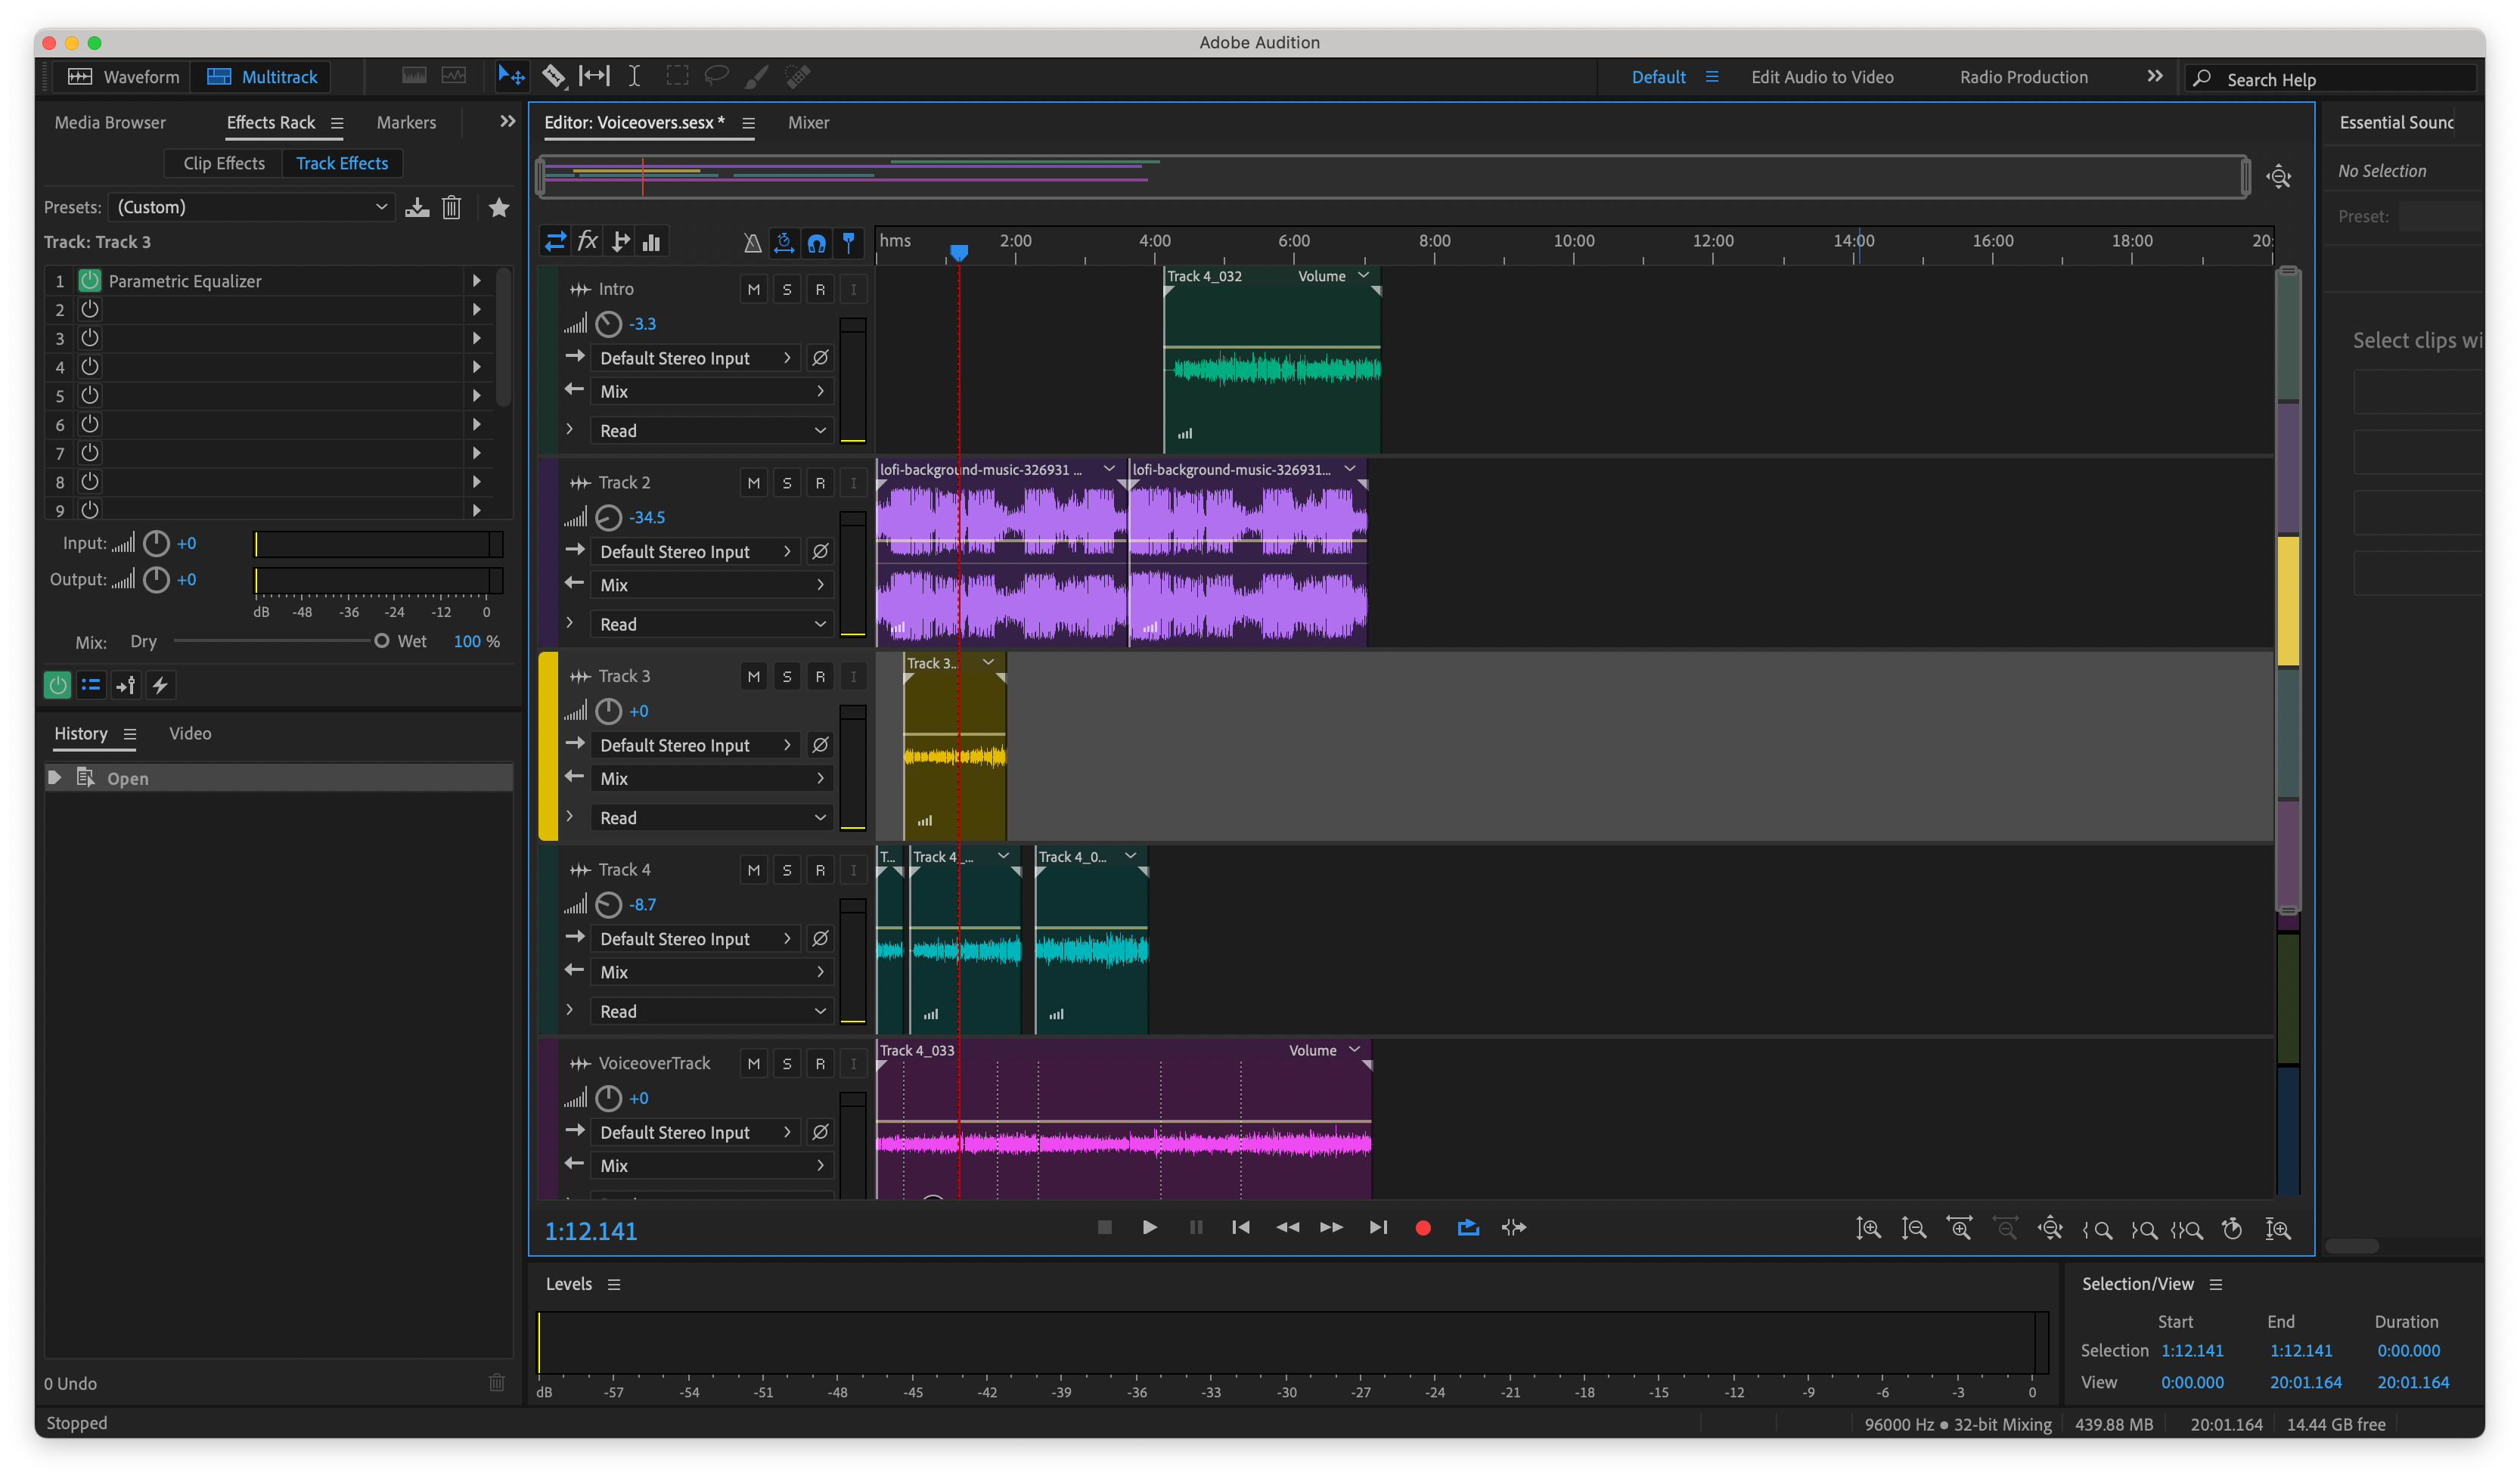
\includegraphics[width=0.6\textwidth]{VideoPresentation/PresentationDevelopment/media/audition.png}
    \caption{Within Adobe Audition, recording the sections of my presentation}
\end{figure}

With my recording completed I then moved over to Premiere Pro to begin editing the video. I first imported my audio files, and then created a new sequence. I then added a nice gradient background which would change colour each time the focus of the presentation changed between the AO levels of the EPQ. I then spent some time finding images and videos to showcase the work I achieved as my voiceover would mention them. To make my video visually appealing I designed some simple animations and transitions between sections, using key frames to animate the position and scale of images and text. I also added some background music to the video, ensuring it was at a low volume so as not to distract from my voiceover and a slow pace to not make the video feel any quicker.

\begin{figure}[H]
    \centering
    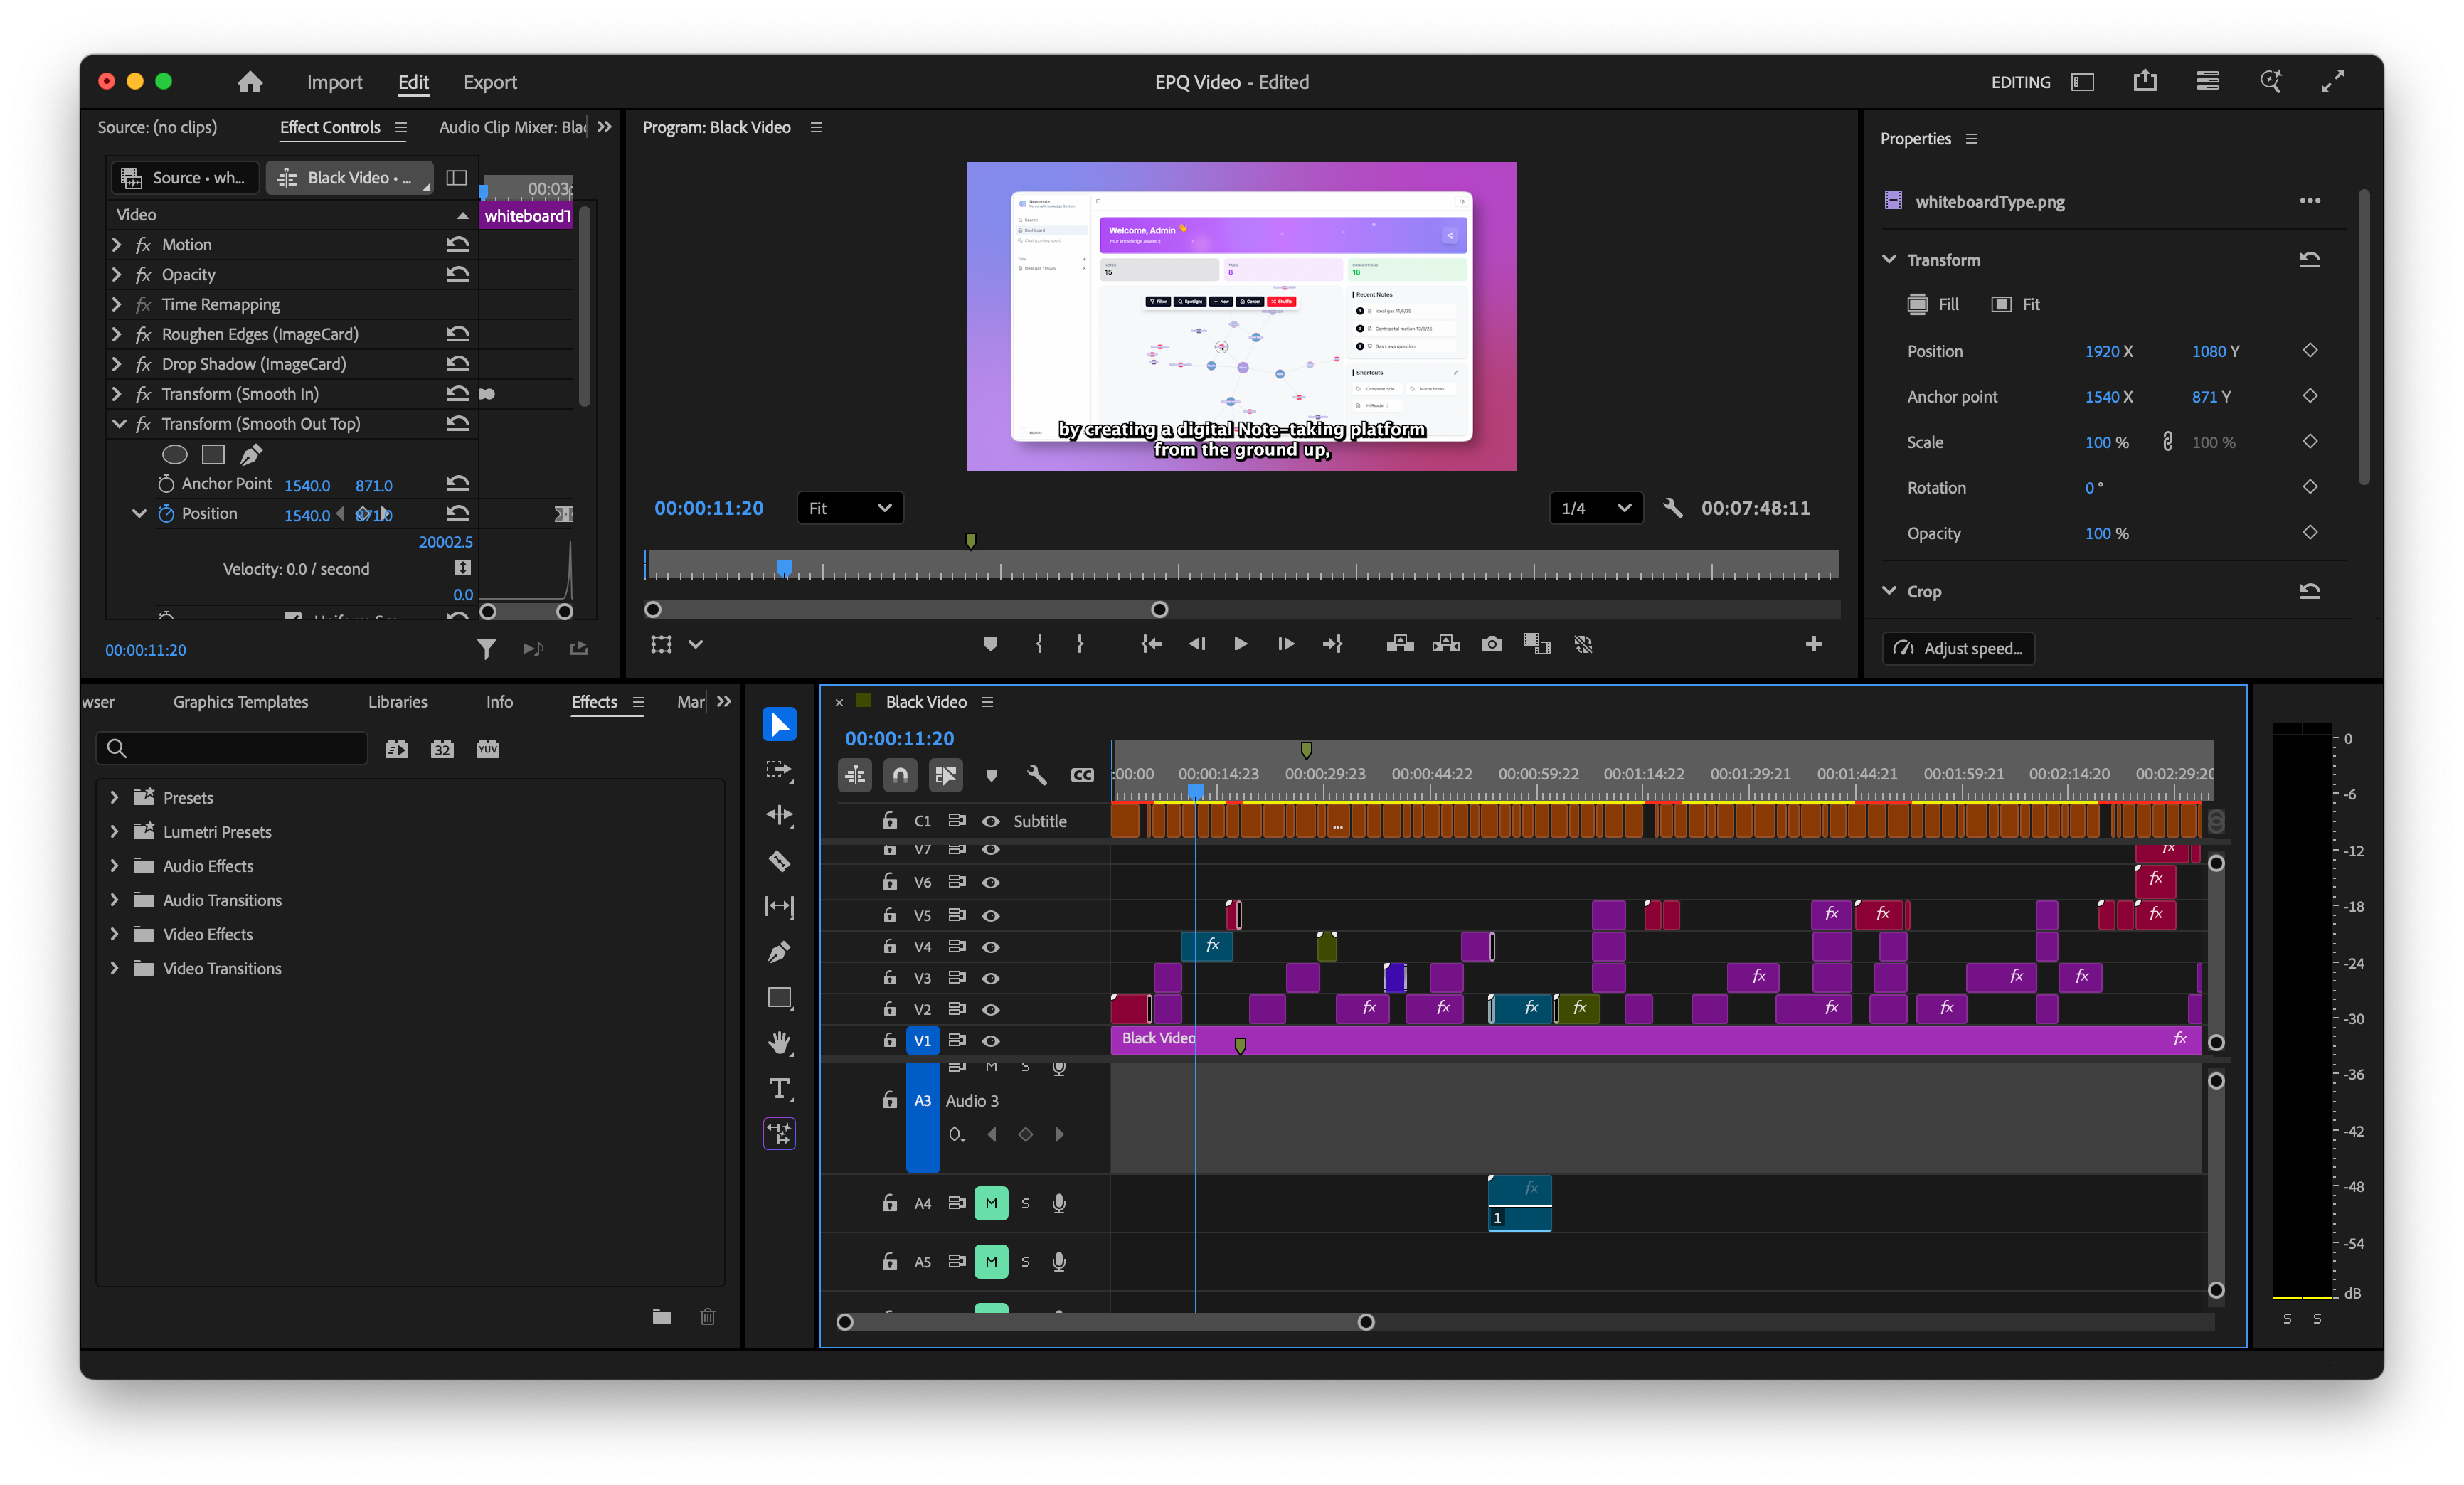
\includegraphics[width=0.6\textwidth]{VideoPresentation/PresentationDevelopment/media/editing.png}
    \caption{Within Premier Pro, editing my presentation video}
\end{figure}

I found the process of animating the video very satisfying, as I was able to use my creativity and skills to showcase my project in a clear, concise and visually appealing manner. 

After spending a couple of days editing the video, I wanted to produce a 'showstopper' moment to end the video on a high. I therefore created a 3D animation in Blender (a software I have some prior experience in) showcasing a conceptual "idea orb" with various neural connections lighting up.

\begin{figure}[H]
    \centering
    \begin{minipage}[t]{0.35\textwidth}
        \centering
        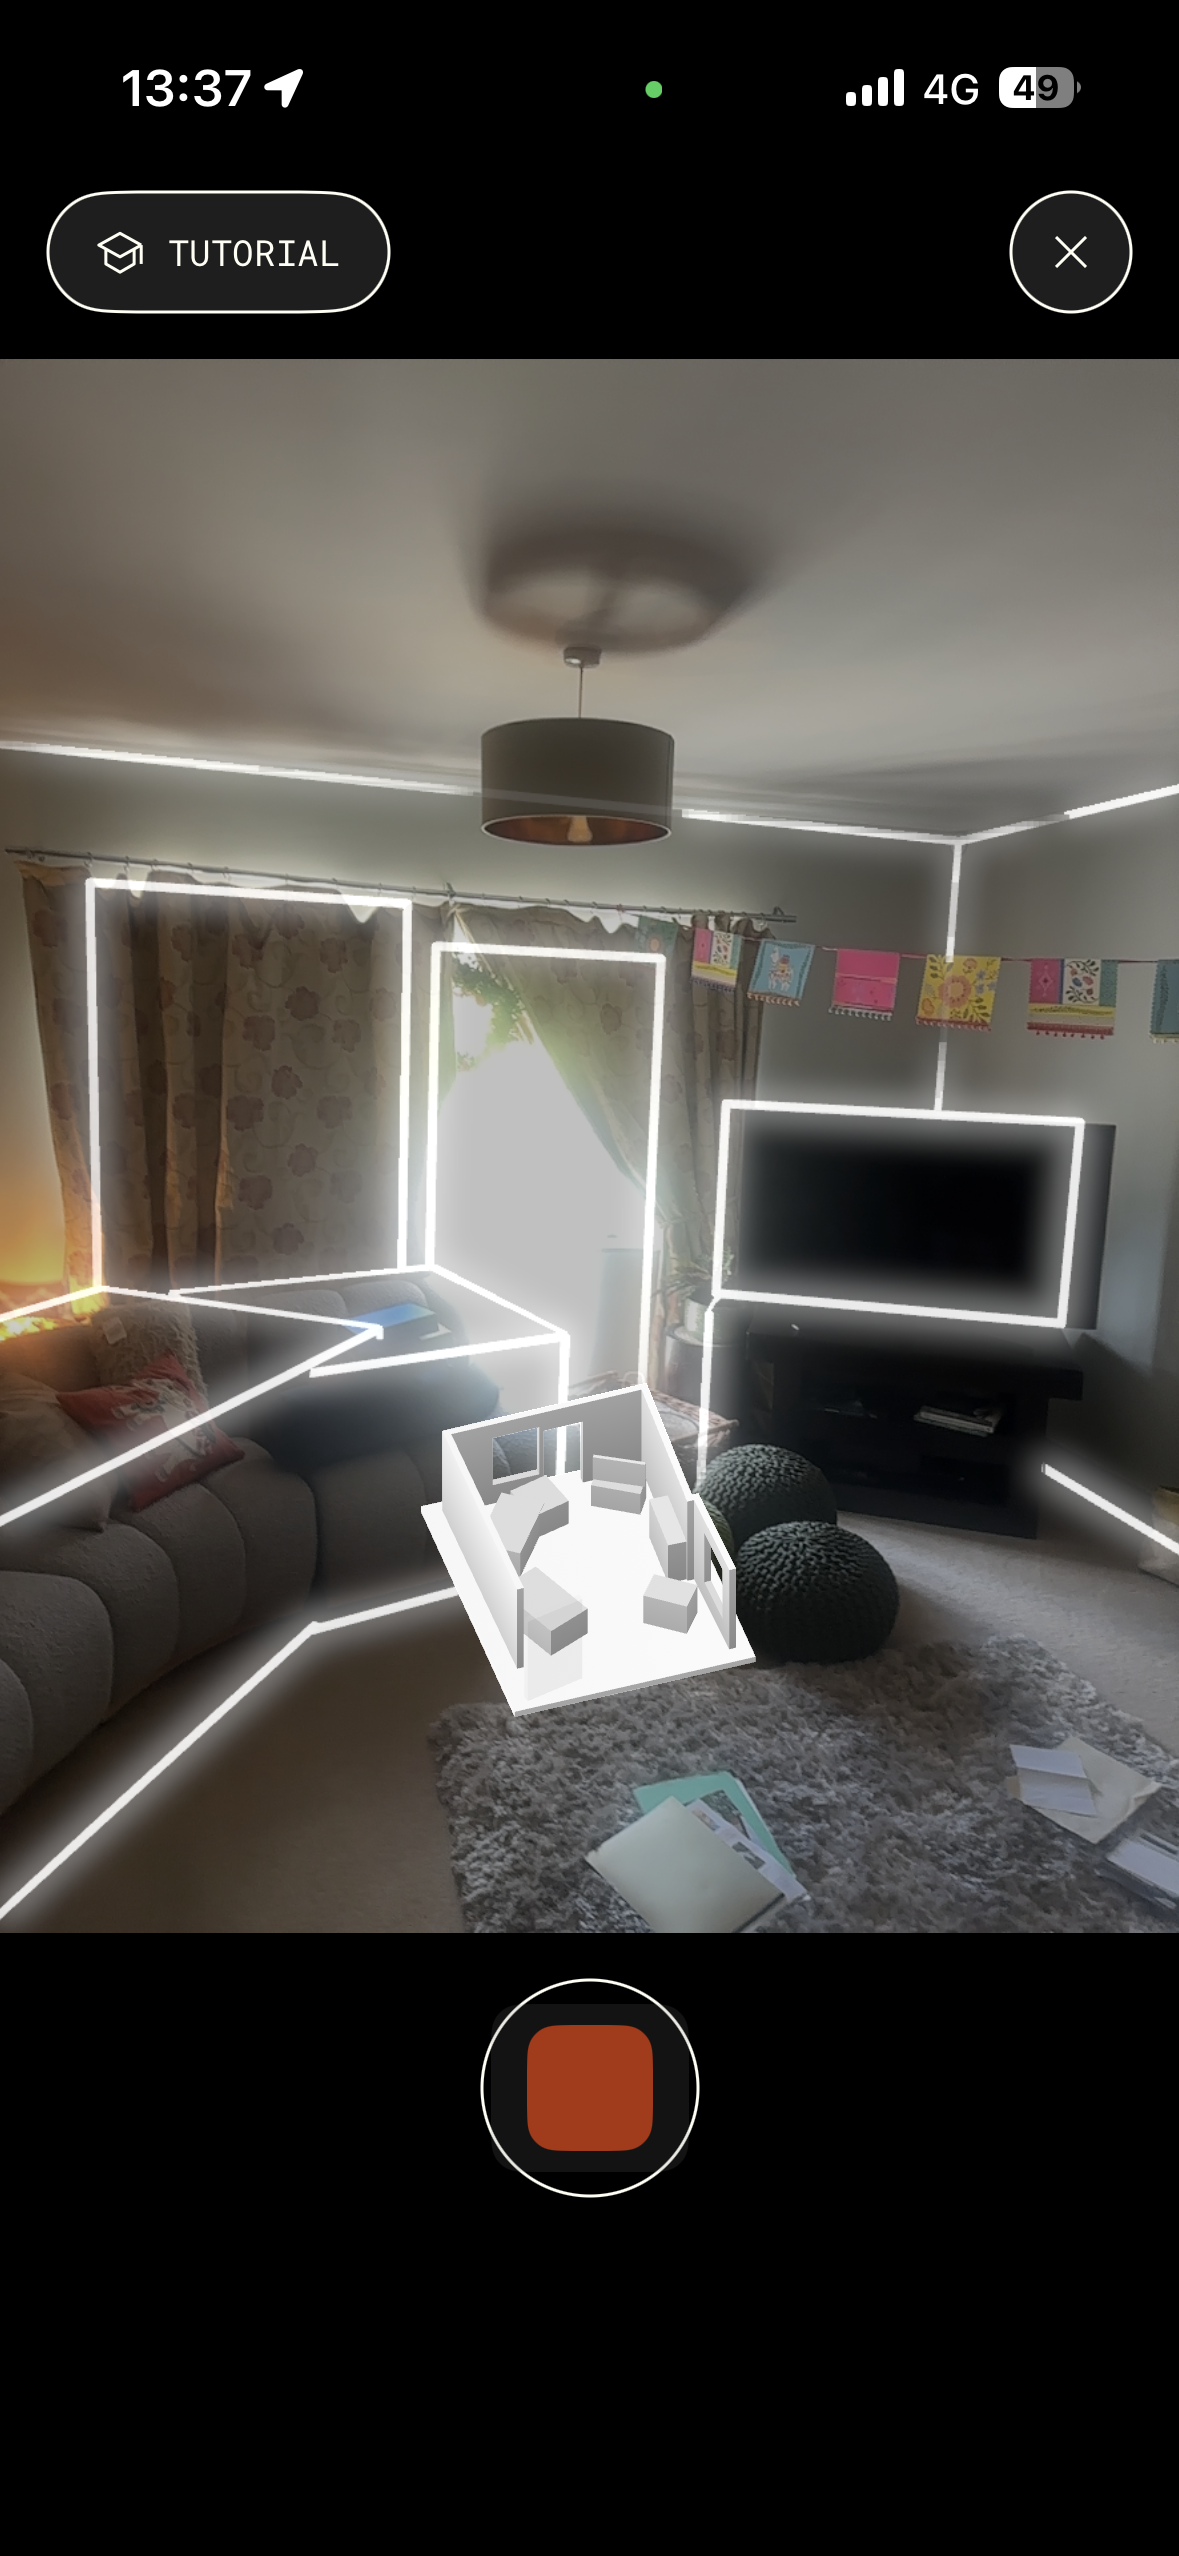
\includegraphics[height=4cm]{VideoPresentation/PresentationDevelopment/media/scanning.png}
        \caption{Scanning my room to create a 3D model for my animation background}
    \end{minipage}%
    \hspace{0.05\textwidth}
    \begin{minipage}[t]{0.6\textwidth}
        \centering
        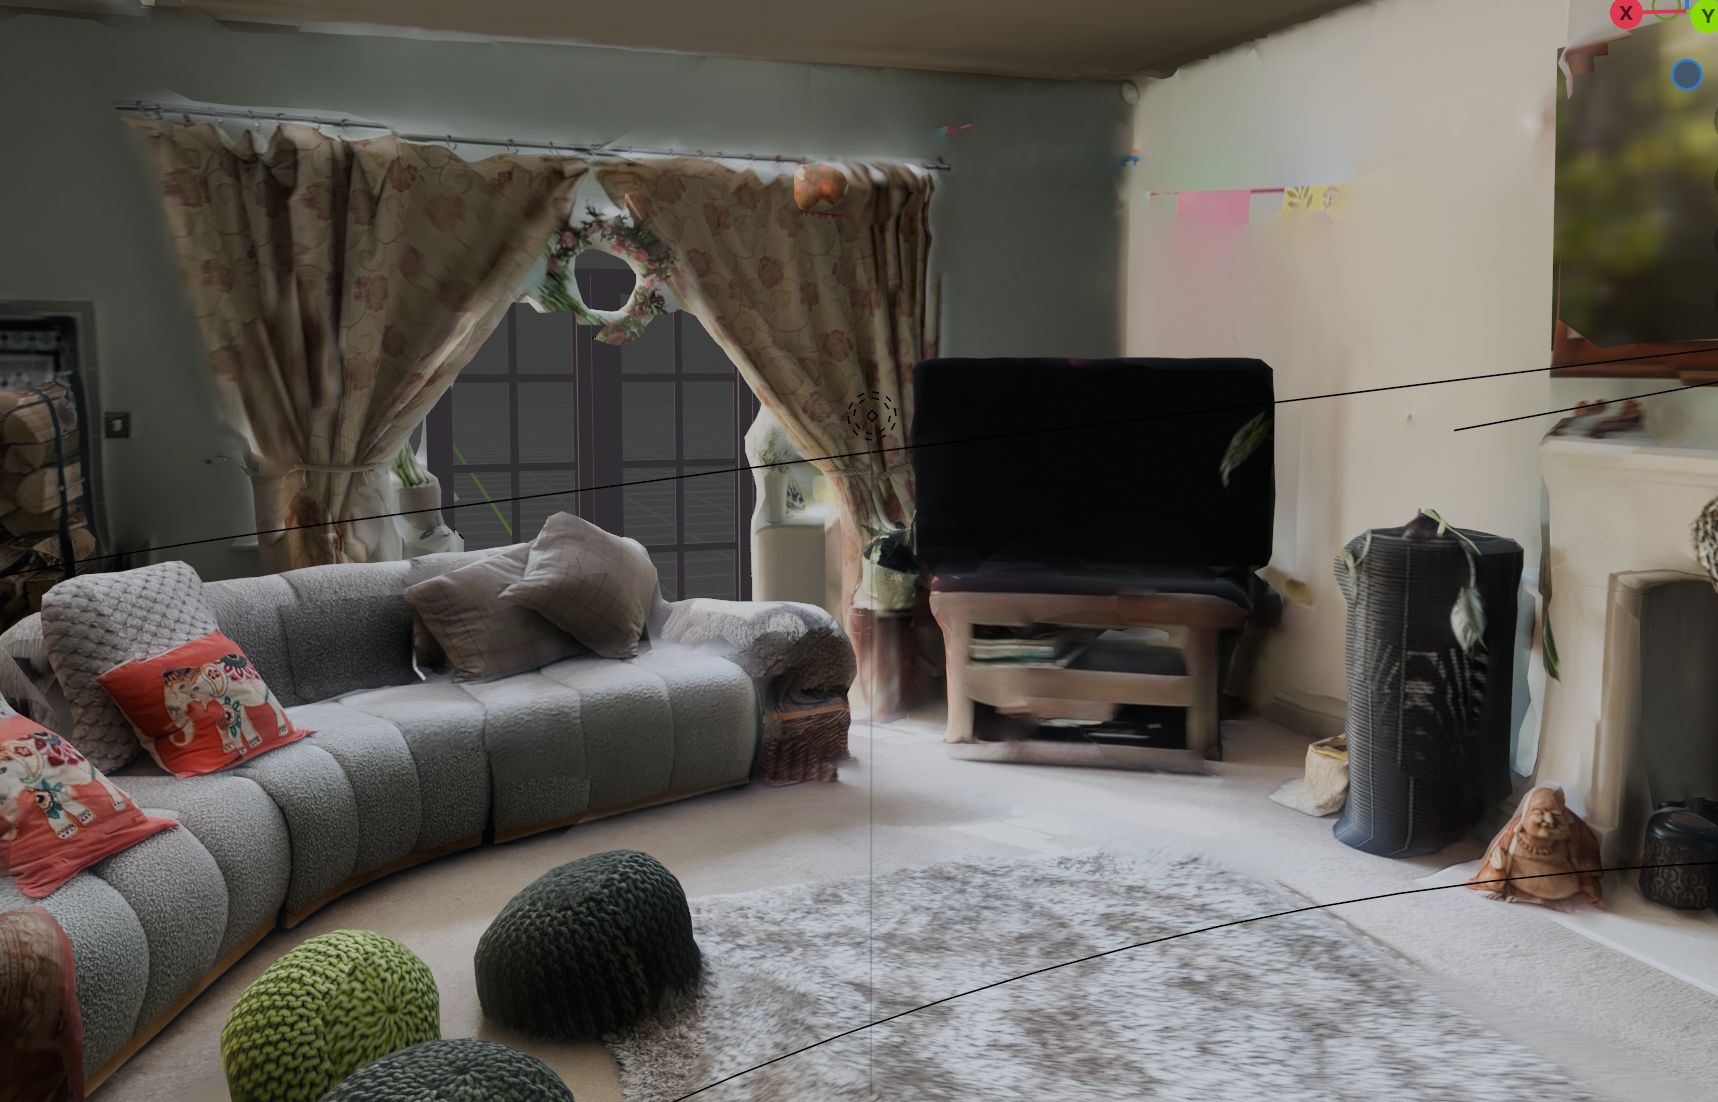
\includegraphics[height=4cm]{VideoPresentation/PresentationDevelopment/media/scanResult.png}
        \caption{The Scan result}
    \end{minipage}
\end{figure}

I therefore spent some time rearranging my Living room to create a suitable background, and then took around 50000 photographs of the scene from different angles ensuring no angle was left uncovered. I processed the images and created a 3D model of my room within my virtual scene. Within Blender I added my "idea orb" models into the scene and animated a 3d camera fly through as the many orbs revealed the name "NeuroNote". 

\begin{figure}[H]
    \centering
    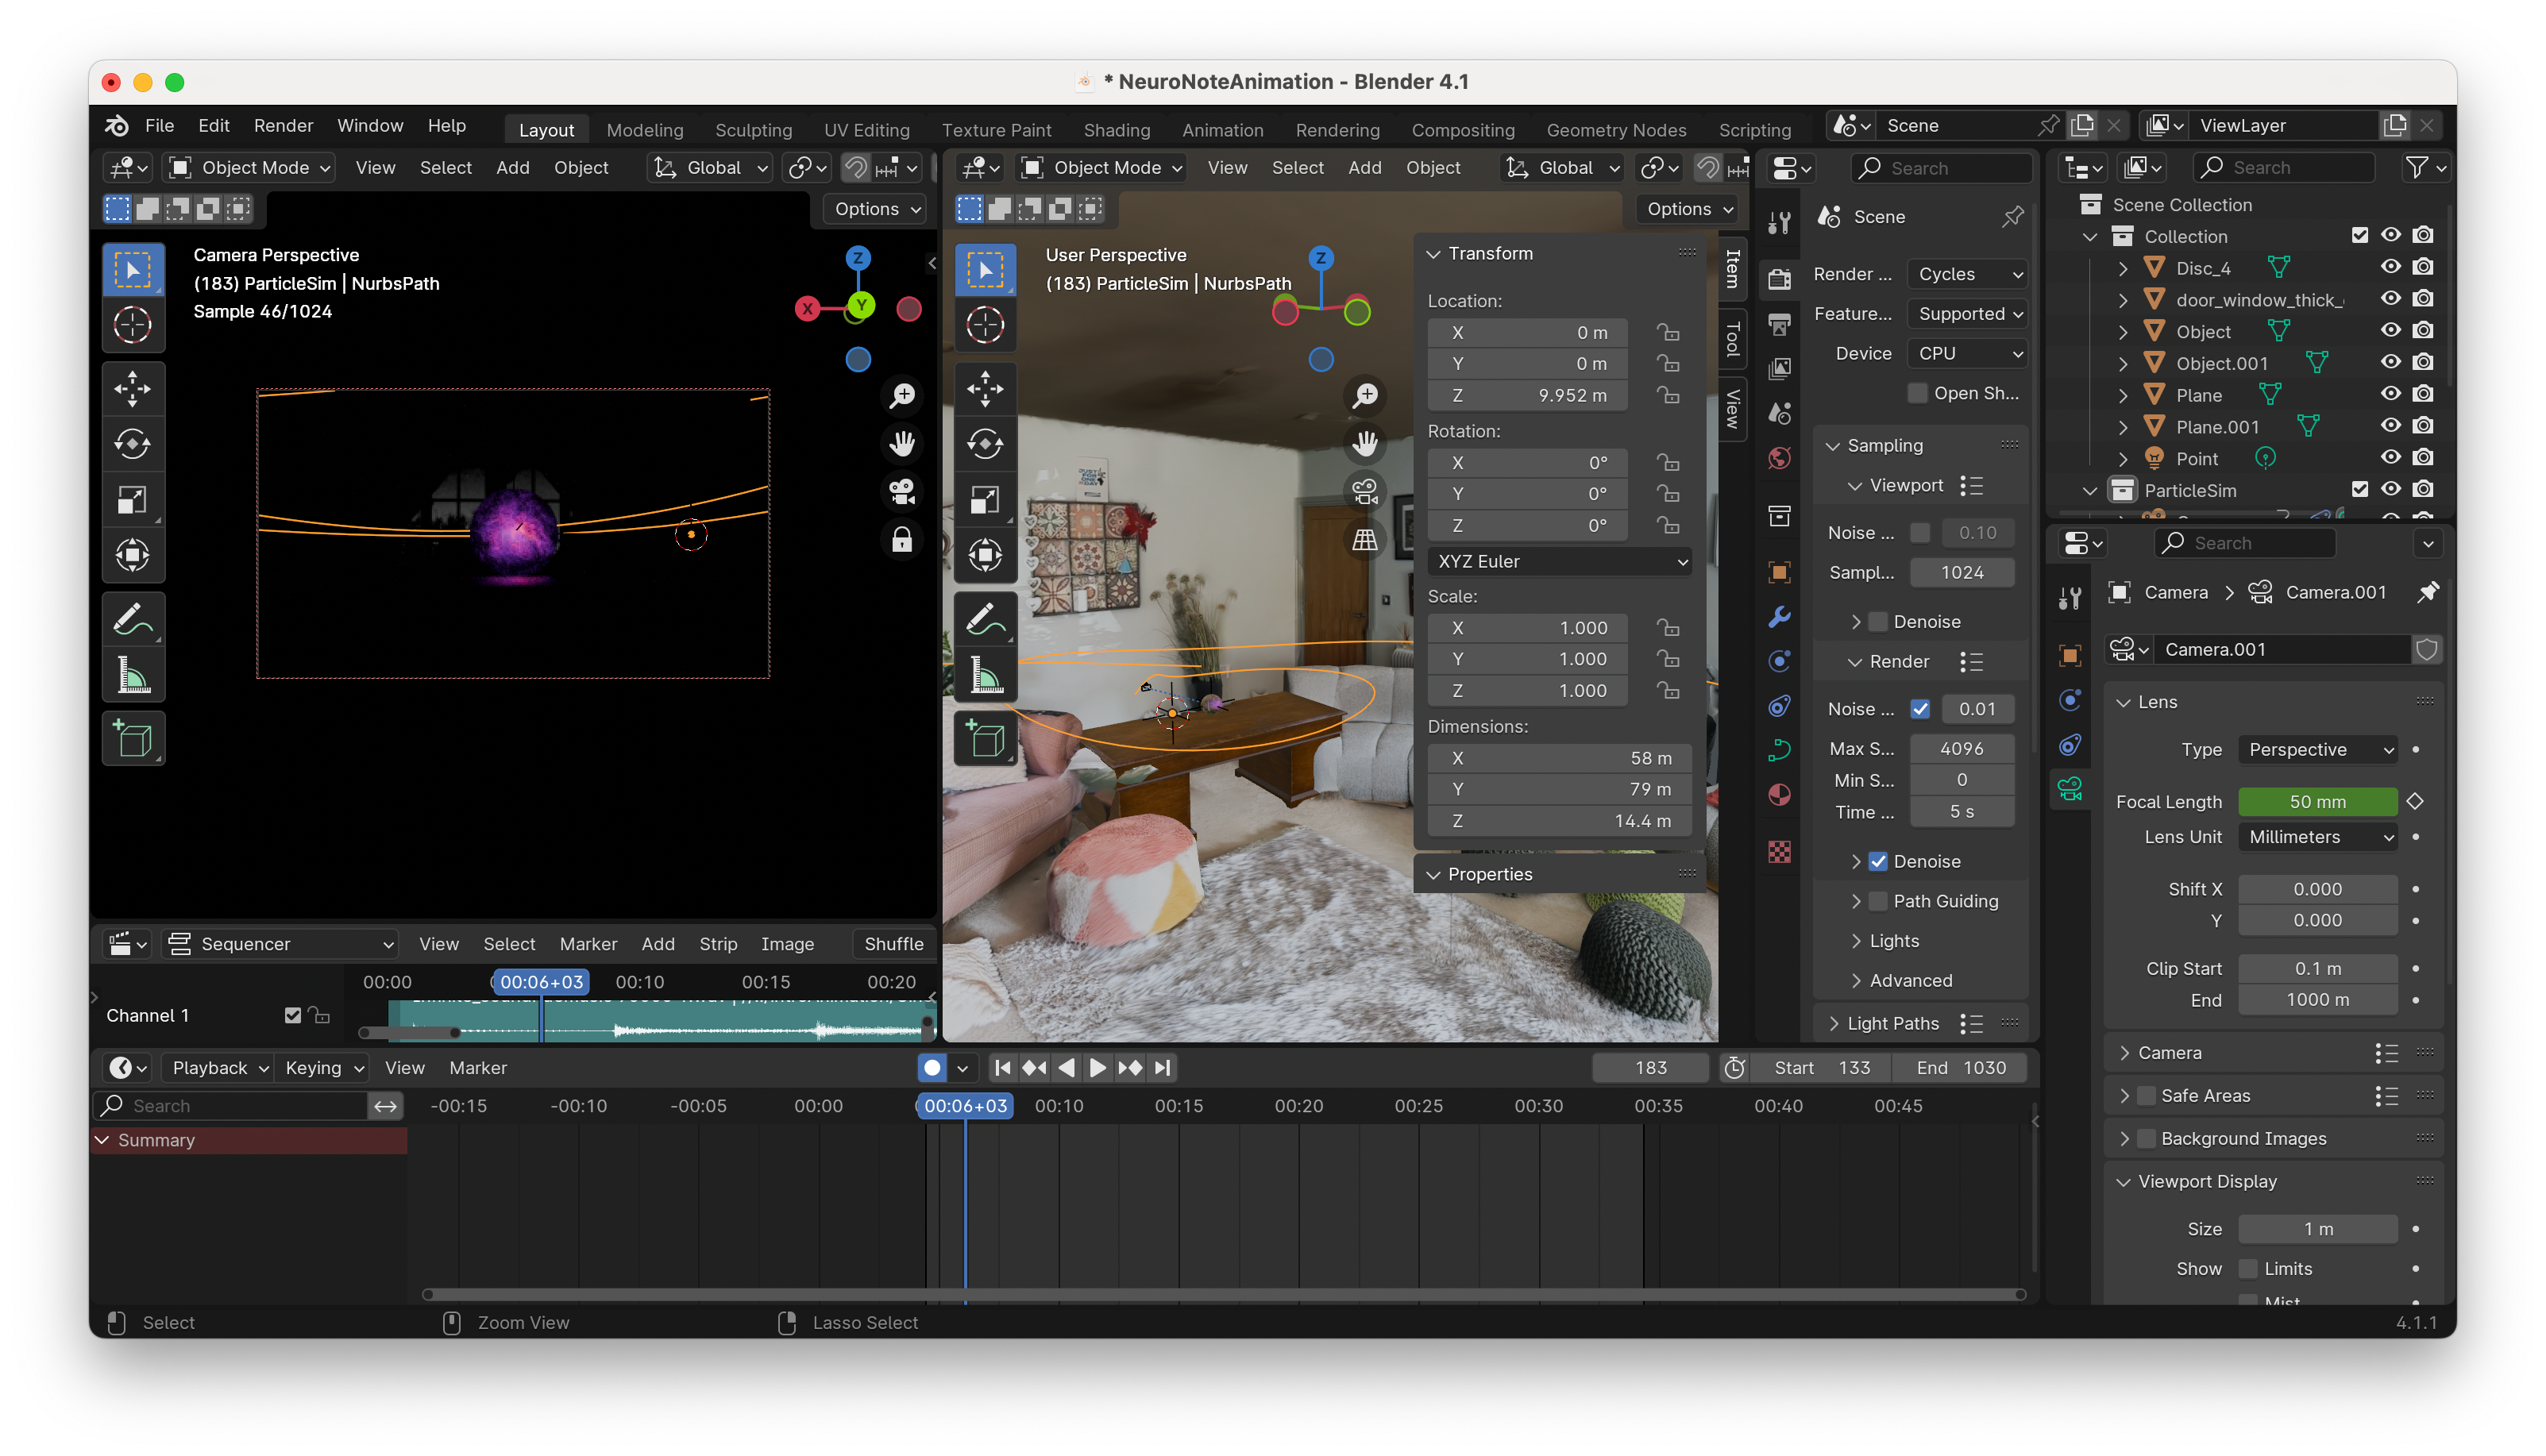
\includegraphics[width=0.6\textwidth]{VideoPresentation/PresentationDevelopment/media/blender.png}
    \caption{Within Blender, Animating my 3D ending}
\end{figure}

I then rendered this animation (which took about 15 hours) and added it to the end of my video, with a final dramatic and spooky voiceover to finish the presentation.

One last addition I made was a Captions track that played alongside the video, further helping to improve understandability and accessibility of the video. As i had already scripted the entire presentation I was able to copy and paste this into Premiere Pro's captioning tool, which automatically synced the captions to my voiceover. After some minor adjustments to the timing of certain captions, I was happy with the final result.

Please Find my presentation attached alongside this report.

I have sent this presentation to a wide array of family and friends who were all very impressed with the quality of the video and the amount of work that had gone into it. Please find my evaluation of the presentation in the Evaluation section of this report in addition to within my PPR.

Many of the techniques I have used here were additionally used to produce my Artifact exploration video which showcases my application in much more detail from a users' perspective.